%!TEX program = xelatex
%!BIB program = bibtex
\documentclass[cn,black,12pt,normal]{elegantnote}
\usepackage{float}
\usepackage{hyperref}
\usepackage{amsmath}
\usepackage{amsfonts}
\usepackage{amssymb}
\usepackage{siunitx}[=v2]
\usepackage{fancyhdr}
\usepackage{newtxtext}
\usepackage{algorithm}
\usepackage{algorithmic}
\newcommand{\uct}[1]{\textsuperscript{\textsuperscript{\cite{#1}}}}
\renewcommand{\tablename}{\textbf{Table}}
\renewcommand{\figurename}{Figure.}
\renewcommand{\refname}{References}
\renewcommand{\contentsname}{Contents}
\renewcommand{\versiontext}{Version: }
\renewcommand{\updatetext}{Update: }
\PassOptionsToPackage{no-math}{fontspec}
\lstset{basicstyle=\footnotesize\ttfamily\color[RGB]{50,0,130},numbers=none,frame=trBL}

\sisetup{mode=text}
\sisetup{range-phrase = \text{ \textasciitilde }}
\pagestyle{fancy}
\fancyhead[L]{School of Software Engineering, Tongji University}
\fancyhead[R]{Data Structure Projects}
\renewcommand{\headrulewidth}{1pt}

\title{Binary Search Tree\\二叉搜索树}
\author{1951510\; 姜文渊}
\institute{\small \url{https://github.com/jwyjohn/Jwy_DataStructureHomework}}
\version{0.50}
\date{\today}

\begin{document}

\maketitle

\textbf{Data structure involved:} Binary search tree, AVL tree

\textbf{Algorithms involved:} Rotation of a binary search tree

\tableofcontents

\newpage

\section{Introduction}

In this project, the author implemented a demo for one variant of binary search trees, the AVL Tree.

A binary search tree (BST), is a rooted binary tree data structure whose internal nodes each store a key greater than all the keys in the node’s left subtree and less than those in its right subtree (i.e. $left<root<right$).\uct{wiki:Binary_search_tree}

Binary search trees allow binary search for fast lookup ($O(log\,n)$ on average), and can be used to implement dynamic sets and lookup tables. In general cases, binary search tree performs searching much faster than the linear time required to find items by key in an (unsorted) array.\uct{wiki:Binary_search_tree}


\section{Demostration}

\subsection{Compile and run the program}

On linux platform with \lstinline{make} and a \lstinline{g++} which supports C++ 11 Standard, just \lstinline{cd} to the \lstinline{./linux} and run \lstinline{make build}. The binary executable will be generated in the same dirctory named as \lstinline{a.out} or \lstinline{avl}, according to the configurations in the \lstinline{Makefile}. Use \lstinline{./a.out} or \lstinline{./avl} to run the program.

The program is an interactive shell, where you can input commands and get results.

Usage of commands can be found on the main screen, and the \lstinline{help} command can give you information about theses commands.  All available commands is listed below.

\begin{enumerate}
    \item \lstinline{help} : Show help for a certain command.
    \item \lstinline{exit} : Exit the program.
    \item \lstinline{init} : Clear and initialize the tree.
    \item \lstinline{add [n1] [n2] [n3] ... } : Add value to the tree (int and >0).
    \item \lstinline{find [n1] [n2] [n3] ... } : Find value in the tree (int and >0).
    \item \lstinline{rm [n1] [n2] [n3] ... } : Remove value from the tree (int and >0).
    \item \lstinline{vlr/lvr/lrv} : Show the tree with different order (Preorder, Inorder and Postorder).
\end{enumerate}
\begin{figure}[H]
    \centering
    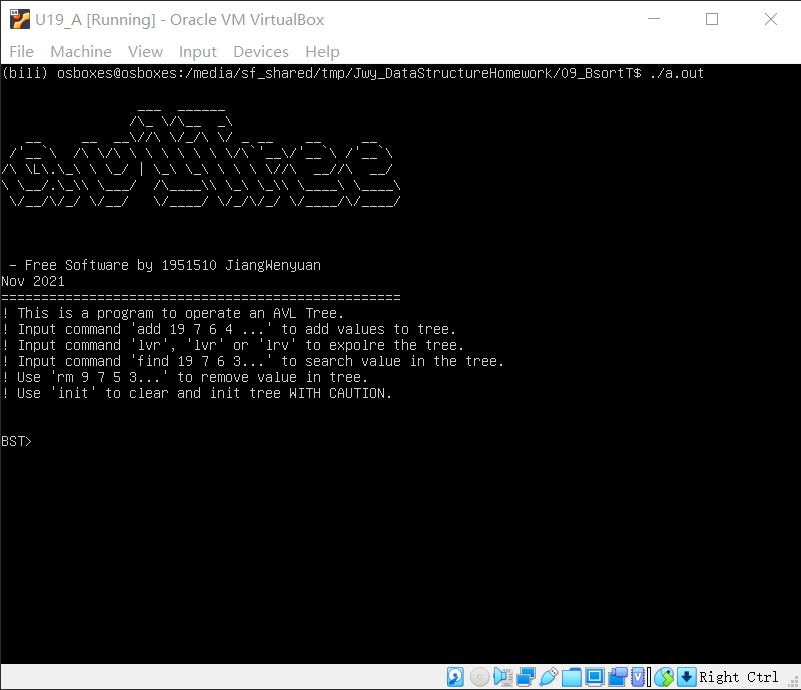
\includegraphics[width=0.7\linewidth]{image/avl_01.jpg}
    \caption{The user interface of the program}
\end{figure}



\subsection{Adding data into the tree}

Use the \lstinline{add [n1] [n2] [n3] ... } command to add data to the tree, as is shown in the figure below.
\begin{figure}[H]
    \centering
    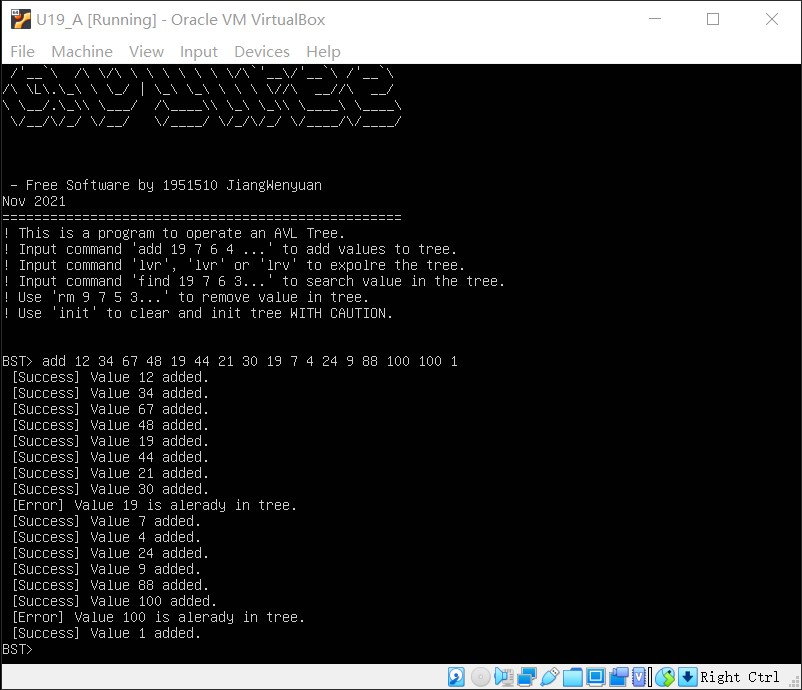
\includegraphics[width=0.7\linewidth]{image/avl_02.jpg}
    \caption{Adding data to the tree}
\end{figure}

\subsection{Inspecting the tree}
Then we could use \lstinline{vlr/lvr/lrv} to inspect the data we previously inputed, as is shown in the figure below.

The inorder traversal of the binary search tree gives an ascending order sequence, which follows the properties of the binary search tree. Observing the other two outputs, we can deduce from the preorder traversal and the inorder traversal that the binary search tree is an AVL tree.
\begin{figure}[H]
    \centering
    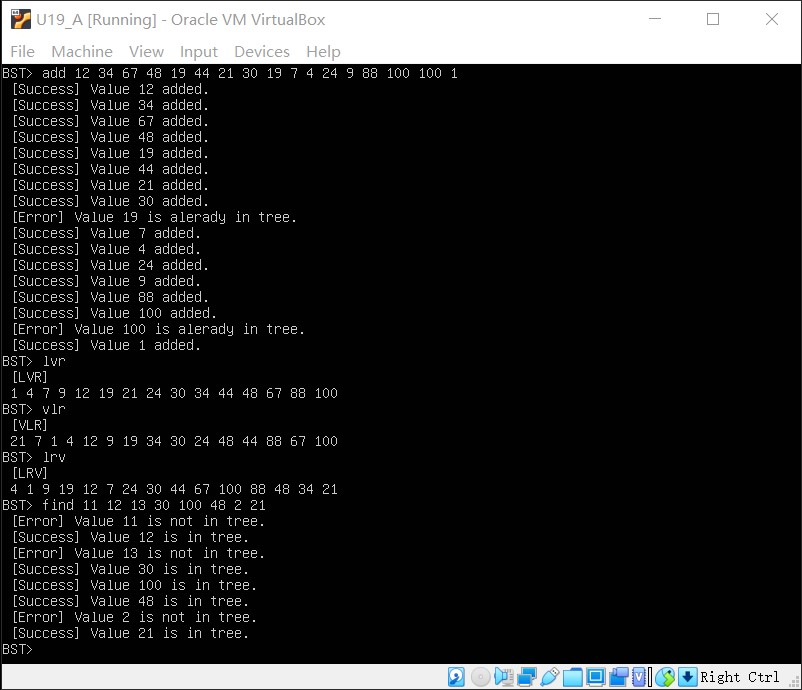
\includegraphics[width=0.7\linewidth]{image/avl_04.jpg}
    \caption{View the tree traversals (Inorder, Preorder and Postorder) and finding elements}
\end{figure}

Also, the \lstinline{find [n1] [n2] [n3] ... } command works correctly when judging whether an element is in the binary search tree.


\subsection{Removing data from the tree}
To remove an element, use \lstinline{rm [n1] [n2] [n3] ... }, as the figure below shows.
\begin{figure}[H]
    \centering
    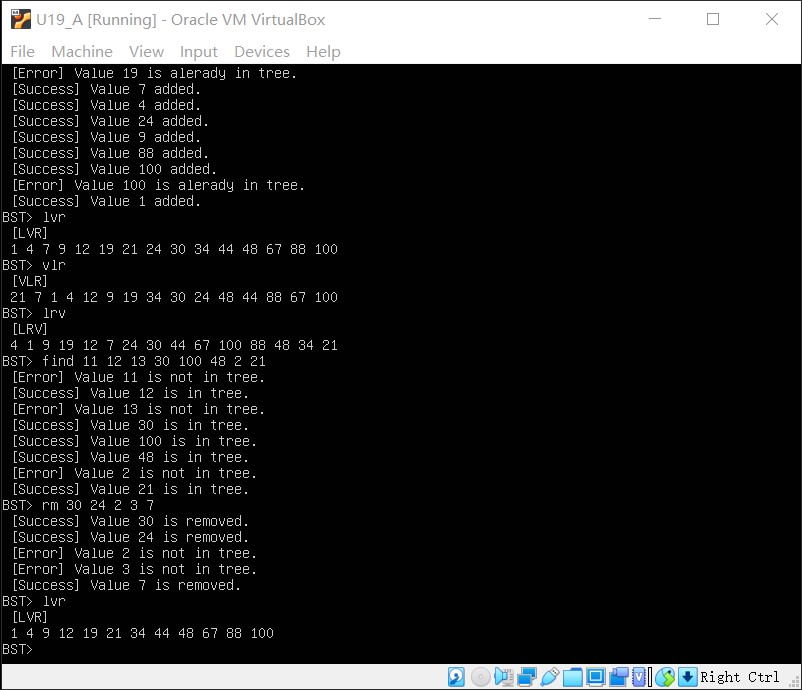
\includegraphics[width=0.7\linewidth]{image/avl_05.jpg}
    \caption{Remove an element is in the tree}
\end{figure}
After removing the element, the properties of the binary search tree remains the same, which can be verified using \lstinline{vlr/lvr/lrv}.

\section{About binary search tree}

\section{Notes on the source code}

If you want to re-use the author's source code in a project, the following are some explaination about the important part of the code. Comments in the source file can provide detailed help, but the following shows the outline.

In the header file \lstinline{main_header.h}, the definition of \lstinline{avl_tree_node} looks like this.
\begin{lstlisting}[language = C++]
typedef struct avl_tree_node
{
	int data = 0;
	int height = 0;
	avl_tree_node *left = nullptr;
	avl_tree_node *right = nullptr;

} avl_tree;
\end{lstlisting}
This is quite straight forward since the \lstinline{data, height} and two subtree pointers are all necessary for an AVL tree.

Then two rotation functions are defined and implemented, followed by the four situations of balancing unbalanced subtrees.
\begin{lstlisting}[language = C++]
avl_tree *rotate_left(avl_tree *t)
{
	avl_tree *root;
	root = t->right;
	t->right = t->right->left;
	root->left = t;
	return root;
};
avl_tree *rotate_right(avl_tree *t)
...
avl_tree *adjust_tree_RR(avl_tree *t)
{
	return rotate_right(t);
};
avl_tree *adjust_tree_LL(avl_tree *t)
...
avl_tree *adjust_tree_LR(avl_tree *t)
{
	avl_tree *root;
	t->left = rotate_left(t->left);
	root = rotate_right(t);
	return root;
};
avl_tree *adjust_tree_RL(avl_tree *t)
...
int balance_node(avl_tree *&t)
...
\end{lstlisting}
A trick here is that the return value type is \lstinline{avl_tree *}, which points to the root node of the adjusted subtree.

After we had the methods to balance a tree, we can consider operations like find, add or remove. These functions are defined like this:
\begin{lstlisting}[language = C++]
avl_tree *find_val(avl_tree *t, int val);
int insert_val(avl_tree *&t, int val);
int remove_val(avl_tree *&t, int val);
\end{lstlisting}
For the convenience of coding, some of these fuctions are recursive, since the data structure of an AVL tree is recursive.

\begin{lstlisting}[language = C++]
int insert_val(avl_tree *&t, int val)
{
	if (t->data == val)
...
	else
	{
		if (val < t->data)
		{
			if (t->left == nullptr)
			{
				avl_tree_node *ins = new avl_tree_node;
				ins->data = val;
				t->left = ins;
			}
			else
			{
				insert_val(t->left, val); // Recursive HERE.
			}
		};
		if (val > t->data)
...
\end{lstlisting}

Also, in the implementation, the author did not consider the situations when some nodes need not to be adjusted in the process after a node is inserted or removed. 

Instead, determination of whether balancing needs to be done is put in the function \lstinline{int balance_node(avl_tree *&t)}, and in the recursive process, after every return of a function, the \lstinline{int balance_node(avl_tree *&t)} is called. This may cause performance loss, but it has been proved that in an AVL tree, the insertion or removal process only needs $O(1)$ balance operations on average, so the performance loss would only be on evaluating \lstinline{if} statements.

\begin{lstlisting}[language = C++]
int insert_val(avl_tree *&t, int val)
{
	if (t->data == val)
	{
        ...
	}
	else
	{
        ...
	};
	balance_node(t);
	return 0;
};
\end{lstlisting}

Detailed implementation of each algorithm follows the textbooks used in this course, and the comments in the code may help you understand how each algorithm actually works. Most of the code in \lstinline{main.cpp} is for processing the user's input, which is not so interesting.

\section{Discussion}

Some other data structures, like hash tables, could achieve a faster speed in searching ($O(1)$), but their usage has many limitations compared with the binary search tree. Also, the \textbf{vanilla} binary search tree (which is the one without modification), can be improved in many ways, to construct more powerful data structures like the famous AVL Tree or the Splay Tree.

A recent improvement involves combination of BST with heap, which can also give us a better performance, which is widely known as \textbf{Treap}s.\uct{yi2005research} An example of Treaps is the \textbf{FHQ-Treap}, which is invented by a Chinese and can perform many operations with the cost $O(log\, n)$.

\newpage
\bibliography{references}
\end{document}
